% Anexo I: tablas y gráficos generados por la notebook de R (did_lanus.R).
\newcommand{\fuente}{\textit{Fuente:} Elaboración propia en base a SEPA (Precios Claros), Secretaría de Industria y Comercio.}
\newcommand{\nota}[1]{\par\medskip\begin{minipage}{\linewidth}\footnotesize\textit{Nota:} #1\par\smallskip\fuente\end{minipage}}

\section*{Anexo I}
\addcontentsline{toc}{section}{Anexo I}

\begin{table}[htbp]
  \caption{Dispersión de precios dentro de la misma cadena y entre cadenas. Total AMBA, diciembre de 2023 y octubre de 2026}
  \label{tab:dispersion}
  \centering\small
  \resizebox{\linewidth}{!}{\begin{tabular}{lcccc}
\toprule
 & \multicolumn{2}{c}{dic-23} & \multicolumn{2}{c}{oct-26} \\
\cmidrule(lr){2-3}\cmidrule(lr){4-5}
 & Distintos partidos & Mismo partido & Distintos partidos & Mismo partido \\
\midrule
\multicolumn{5}{l}{\textit{Panel A. Misma cadena}} \\
Cantidad de precios idénticos (\%) & 68,84 & 76,77 & 83,94 & 89,96 \\
Diferencia de precios mediana (\%) & 0,52 & 0,30 & 0,17 & 0,07 \\
Diferencia de precios promedio (\%) & 1,43 & 1,23 & 0,43 & 0,28 \\
Desvío de precios (\%) & 3,16 & 3,08 & 1,68 & 1,34 \\
SKUs comparados & 14.468 & 14.468 & 40.036 & 40.028 \\
\midrule
\multicolumn{5}{l}{\textit{Panel B. Entre cadenas del mismo formato}} \\
Cantidad de precios idénticos (\%) & 7,39 & 12,83 & 29,14 & 30,50 \\
Diferencia de precios mediana (\%) & 6,64 & 6,11 & 2,12 & 1,75 \\
Diferencia de precios promedio (\%) & 9,78 & 8,91 & 3,09 & 2,56 \\
Desvío de precios (\%) & 13,66 & 12,37 & 4,98 & 4,17 \\
SKUs comparados & 9.937 & 9.808 & 15.821 & 15.627 \\
\bottomrule
\end{tabular}
}
  \nota{Panel A: mismo producto en la misma cadena; cada formato de local (por ejemplo, Carrefour Express o Disco) se compara
  contra sí mismo entre partidos (distintos partidos) y dentro de cada partido (mismo partido). Cadena = promedio de sus
  formatos. Panel B: mismo producto en distintas cadenas del mismo formato: supermercados (DIA, Carrefour Express, Carrefour
  Market, Disco y SuperChangomas) contra supermercados e hipermercados (Coto, Carrefour Hiper, Jumbo, Vea, Changomas e
  HiperChangomas) contra hipermercados; el precio de cada cadena se compara con el promedio de las cadenas de su formato que
  venden ese producto, en el mismo partido o en el conjunto del AMBA. Sin Maxi ni Lanús. Total = promedio de las cadenas.
  Precios idénticos: diferencia de hasta \(\pm\)0,25\%.}
\end{table}

\begin{figure}[htbp]
  \caption{Precios en Lanús y en el resto del AMBA: hipermercados y supermercados}
  \label{fig:tendencias}
  \centering
  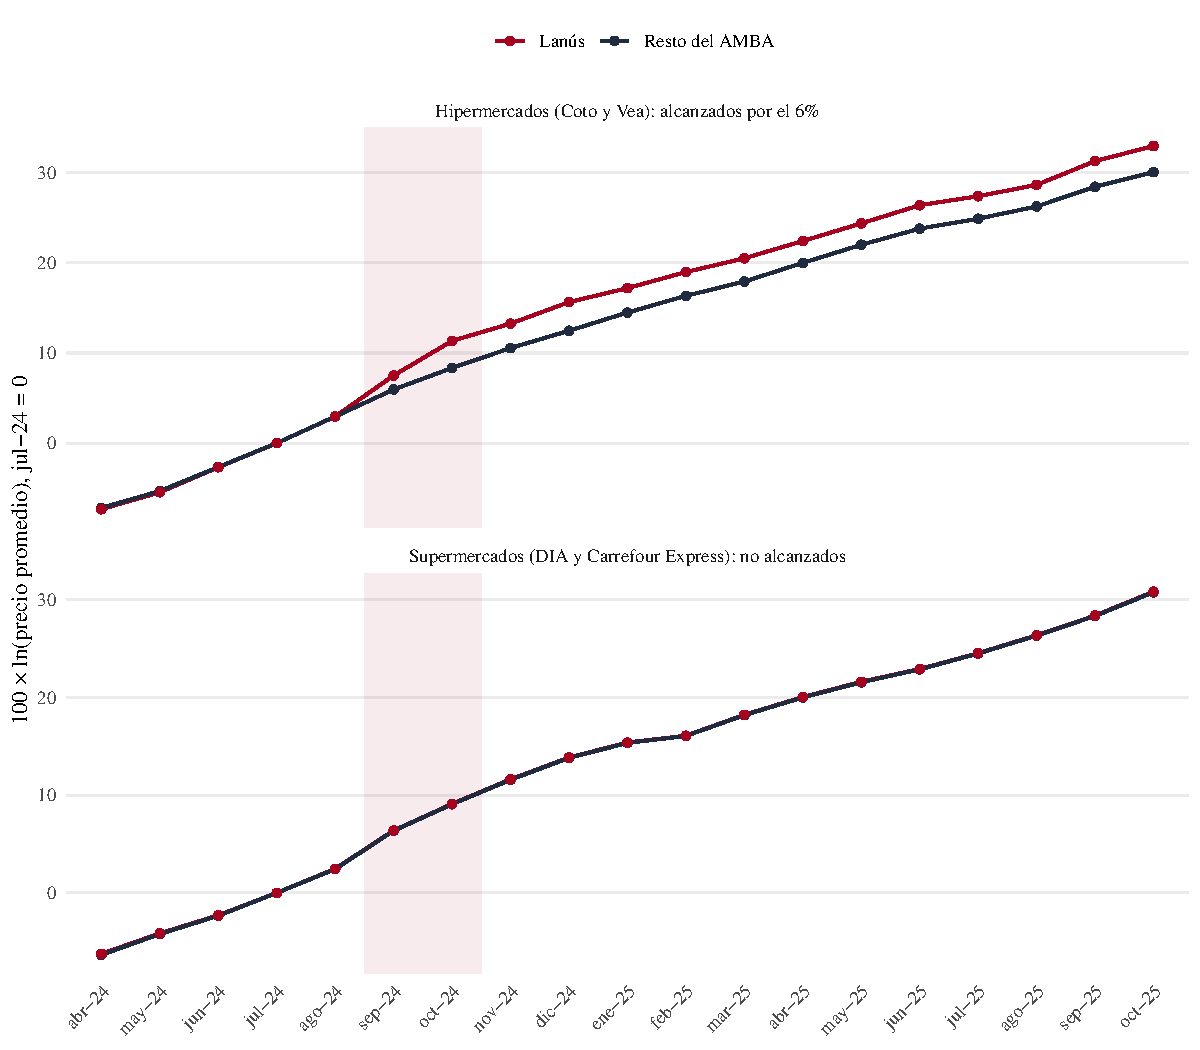
\includegraphics[width=0.65\linewidth]{figuras/tendencias.pdf}
  \nota{100 \(\times\) logaritmo del precio promedio de la canasta de cada formato, julio de 2024 = 0. Mismo producto y mismo
  formato de local; para el resto del AMBA se promedia entre partidos y los formatos tienen igual peso. La franja sombreada
  marca septiembre y octubre de 2024.}
\end{figure}

\begin{table}[htbp]
  \caption{Efecto del aumento de la tasa sobre los precios de los hipermercados de Lanús}
  \label{tab:did}
  \centering\small
  \begin{tabular}{lcccc}
\toprule
 & (1) & (2) & (3) & (4) \\
 & Hipermercados & Hipermercados & Coto & Vea \\
\midrule
Lanús $\times$ Post & 3,52 & 3,22 & 3,42 & 2,30 \\
 & (0,09) & (0,05) & (0,06) & (0,10) \\
p-valor de permutación & & 0,048 & 0,048 & 0,125 \\
\midrule
EF unidad & Sí & Sí & Sí & Sí \\
EF mes & Sí & & & \\
EF producto$\times$formato$\times$mes & & Sí & Sí & Sí \\
Partidos & 21 & 21 & 21 & 8 \\
Observaciones & 980.305 & 980.305 & 898.569 & 81.736 \\
Traslado (\%) & & 83 & 89 & 59 \\
\bottomrule
\end{tabular}

  \nota{estimación de la ecuación~\eqref{eq:2}. Variable dependiente: 100 \(\times\) ln(precio). Errores estándar agrupados
  por producto entre paréntesis. El p-valor de permutación se calcula según la sección~5. Ventana: abril de 2024 a octubre
  de 2025, sin agosto ni septiembre de 2024. Traslado = efecto estimado / 3,86. EF: efectos fijos.}
\end{table}

\begin{table}[htbp]
  \caption{Estudio de eventos: hipermercados de Lanús}
  \label{tab:es}
  \centering\small
  \begin{tabular}{lcc|lcc}
\toprule
Mes & $\delta_k$ & (e.e.) & Mes & $\delta_k$ & (e.e.) \\
\midrule
abr-24 & -0,10 & (0,03) & feb-25 & 3,24 & (0,09) \\
may-24 & -0,09 & (0,02) & mar-25 & 3,14 & (0,07) \\
jun-24 & 0,02 & (0,02) & abr-25 & 3,14 & (0,07) \\
jul-24 & 0,00 & ref. & may-25 & 3,20 & (0,08) \\
ago-24 & 0,04 & (0,02) & jun-25 & 3,26 & (0,08) \\
sep-24 & 1,49 & (0,05) & jul-25 & 3,14 & (0,07) \\
oct-24 & 3,03 & (0,05) & ago-25 & 3,00 & (0,06) \\
nov-24 & 3,17 & (0,07) & sep-25 & 3,13 & (0,06) \\
dic-24 & 3,35 & (0,07) & oct-25 & 3,19 & (0,06) \\
ene-25 & 3,24 & (0,08) &  & &  \\
\bottomrule
\end{tabular}

  \nota{estimación de la ecuación~\eqref{eq:6}. Coeficientes en puntos porcentuales; referencia: julio de 2024. Errores
  estándar agrupados por producto entre paréntesis.}
\end{table}

\begin{figure}[htbp]
  \caption{Estudio de eventos: hipermercados de Lanús}
  \label{fig:es}
  \centering
  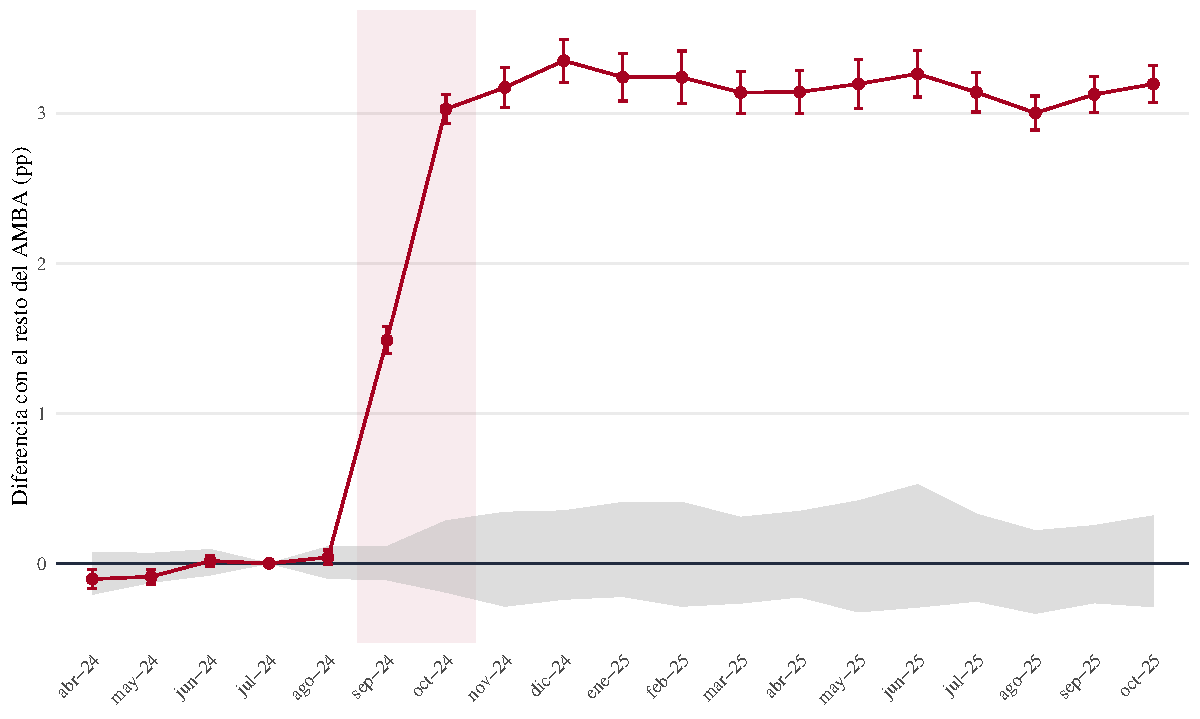
\includegraphics[width=0.85\linewidth]{figuras/event_study.pdf}
  \nota{coeficientes de la ecuación~\eqref{eq:6} con intervalos de confianza del 95\% (errores agrupados por producto);
  referencia: julio de 2024. La franja gris muestra el rango de coeficientes que se obtiene al asignar el tratamiento a cada
  uno de los demás partidos. La franja sombreada marca septiembre y octubre de 2024.}
\end{figure}

\begin{figure}[htbp]
  \caption{Inferencia por permutación: efecto estimado al asignar el tratamiento a cada partido}
  \label{fig:perm}
  \centering
  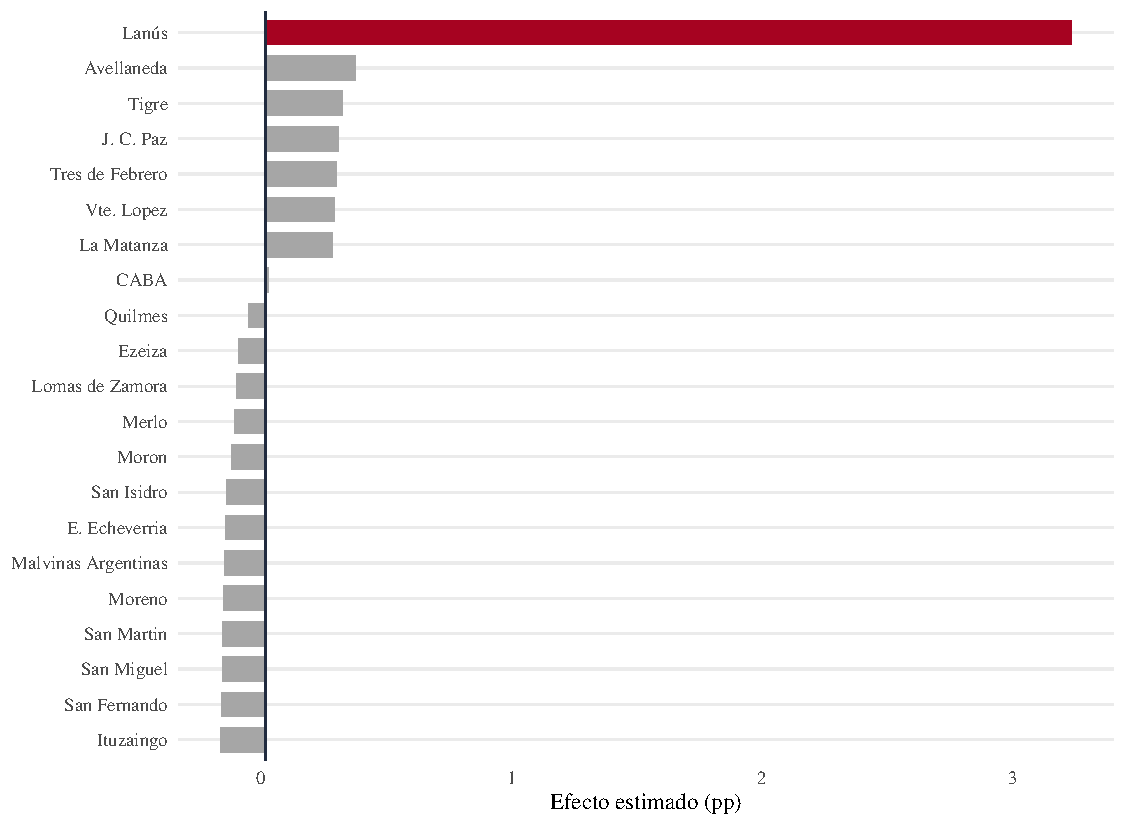
\includegraphics[width=0.68\linewidth]{figuras/permutacion.pdf}
  \nota{hipermercados (Coto y Vea). Cada barra es el coeficiente de la ecuación~\eqref{eq:2} estimado asignando el
  tratamiento al partido indicado, sin Lanús en la muestra de control. P-valor de permutación de Lanús: 0,048.}
\end{figure}

\begin{table}[htbp]
  \caption{Prueba placebo: supermercados de Lanús (no alcanzados por el aumento)}
  \label{tab:placebo}
  \centering\small
  \begin{tabular}{lccc}
\toprule
Supermercados & $\hat\delta$ (pp) & (e.e.) & p-valor de permutación \\
\midrule
Total (DIA y Carrefour Express) & -0,02 & (0,01) & 0,667 \\
DIA & -0,02 & (0,01) & 0,625 \\
Carrefour Express & -0,02 & (0,02) & 0,818 \\
\bottomrule
\end{tabular}

  \nota{estimación de la ecuación~\eqref{eq:2} para los supermercados de Lanús (DIA y Carrefour Express), comparados con
  los mismos formatos en el resto del AMBA. Errores estándar agrupados por producto entre paréntesis.}
\end{table}

\begin{figure}[htbp]
  \caption{Prueba placebo: estudio de eventos para los supermercados de Lanús}
  \label{fig:es_placebo}
  \centering
  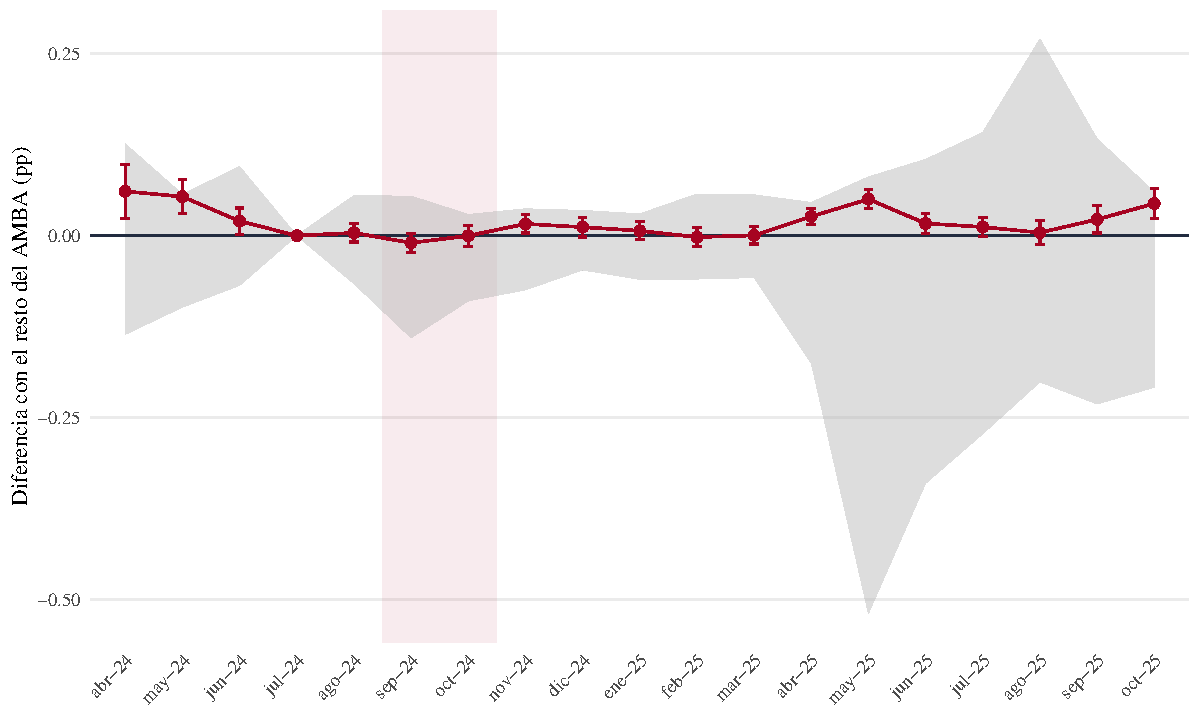
\includegraphics[width=0.85\linewidth]{figuras/event_study_placebo.pdf}
  \nota{coeficientes de la ecuación~\eqref{eq:6} estimada para los supermercados (DIA y Carrefour Express), con intervalos
  de confianza del 95\% (errores agrupados por producto); referencia: julio de 2024. La franja gris muestra el rango de
  coeficientes de los demás partidos.}
\end{figure}
